\documentclass{standalone}
\usepackage{tikz}
\usetikzlibrary{shapes.geometric}
\begin{document}
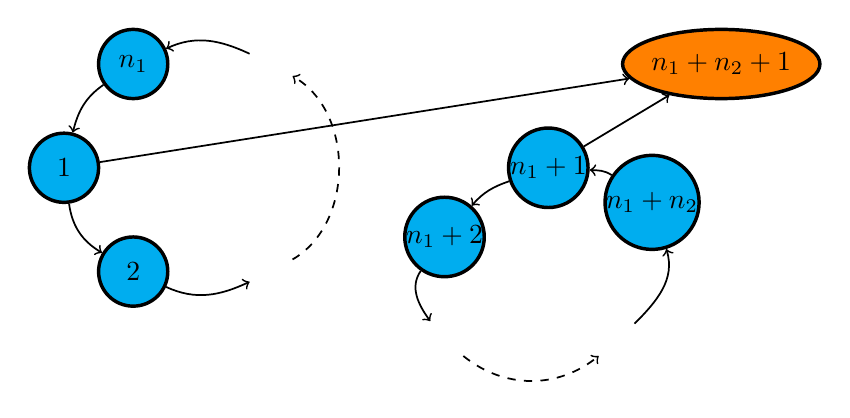
\begin{tikzpicture}
[every node/.style={inner sep=0pt}]
\node (4) [circle, minimum size=25.0pt, fill=cyan, line width=1.25pt, draw=black] at (50.0pt, -25.0pt) {\textcolor{black}{$n_1$}};
\node (1) [circle, minimum size=25.0pt, fill=cyan, line width=1.25pt, draw=black] at (25.0pt, -62.5pt) {\textcolor{black}{1}};
\node (2) [circle, minimum size=25.0pt, fill=cyan, line width=1.25pt, draw=black] at (50.0pt, -100.0pt) {\textcolor{black}{2}};
\node (11) [circle, minimum size=16.25pt, fill=white, line width=1.25pt] at (100.0pt, -25.0pt)  {};
\node (3) [circle, minimum size=16.25pt, fill=white, line width=1.25pt] at (100.0pt, -100.0pt)  {};
\node (5) [circle, minimum size=25.0pt, fill=cyan, line width=1.25pt, draw=black] at (200.0pt, -62.5pt) {\textcolor{black}{$n_1+1$}};
\node (9) [circle, minimum size=16.25pt, fill=white, line width=1.25pt] at (162.5pt, -125.0pt)  {};
\node (8) [ellipse, minimum size=25.0pt, fill=orange, line width=1.25pt, draw=black] at (262.5pt, -25.0pt) {\textcolor{black}{$n_1+n_2+1$}};
\node (6) [circle, minimum size=25.0pt, fill=cyan, line width=1.25pt, draw=black] at (162.5pt, -87.5pt) {\textcolor{black}{$n_1+2$}};
\node (10) [circle, minimum size=16.25pt, fill=white, line width=1.25pt] at (225.0pt, -125.0pt)  {};
\node (7) [circle, minimum size=25.0pt, fill=cyan, line width=1.25pt, draw=black] at (237.5pt, -75.0pt) {\textcolor{black}{$n_1+n_2$}};
\draw [line width=0.625, ->, color=black] (4) to  [in=76, out=215] (1);
\draw [line width=0.625, ->, color=black] (1) to  [in=149, out=278] (2);
\draw [line width=0.625, ->, color=black] (2) to  [in=205, out=335] (3);
\draw [line width=0.625, ->, dashed, color=black] (3) to  [in=330, out=30] (11);
\draw [line width=0.625, ->, color=black] (11) to  [in=25, out=155] (4);
\draw [line width=0.625, ->, color=black] (1) to  (8);
\draw [line width=0.625, ->, color=black] (5) to  (8);
\draw [line width=0.625, ->, color=black] (5) to  [in=49, out=199] (6);
\draw [line width=0.625, ->, color=black] (6) to  [in=126, out=235] (9);
\draw [line width=0.625, ->, color=black] (10) to  [in=287, out=45] (7);
\draw [line width=0.625, ->, color=black] (7) to  [in=357, out=146] (5);
\draw [line width=0.625, ->, dashed, color=black] (9) to  [in=219, out=321] (10);
\end{tikzpicture}

\end{document}
